\chapter{Aspects for further standardisation activities}
In this chapterr various aspects of the subject oriented modelling and programming concept are outlined. These aspects are already published on different confernces. The following sections are based on these publications.
The concepts described in theses sections will be part of future standardisation activities.

\section{Subjects and Shared Input Pools}

Shared input pools have the same structure like subject-specific ones, and thus, the same properties like the standard input pool. The only difference is that different subjects can deposit in or remove messages from a shared input pool. Subjects that want to send a message via a shared input pool do not use a subject name as addressee of a message, but the name of a shared input pool instead. In a distributed system several shared input pools for different purposes can be used. Figure 7 shows the slightly changed structure of the traffic management system when operating it with a shared input pool. The subject "Car detection" represents the shared input pool.


Figure 7: Traffic Management System with Shared Input Pool

\begin{figure}
	\centering
	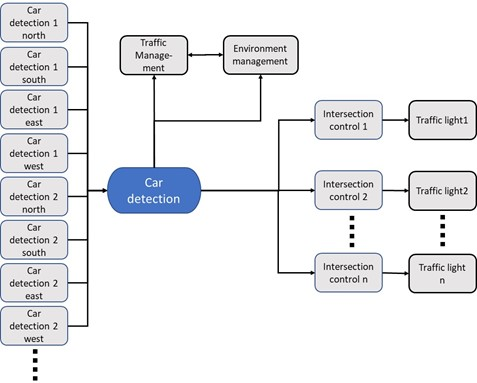
\includegraphics[width=0.7\linewidth]{Figures/Chapter5/figuresshared/SharedInputPoolExample.jpg}
	\caption[Traffic Management System with Shared Input Pool]{Traffic Management System with Shared Input Pool}
	\label{fig:SharedInputPooTraffic}
\end{figure}


Shared input pools make a distributed system more flexible when additional participants or nodes are added. For instance, a third intersection control could be added to the traffic management system without much effort. In this case, only the additional detectors and the components for controlling the intersection have to be complemented and linked to the shared input pool. The extension would have no impact on the behavior of the other subjects and their behavior in that system.
There is one additional attribute for shared input pool: It defines whether a message will be removed from the input pool once a message has been picked up by a receiving subject. This mechanism is required, since several subject may need to process a particular message. In addition, it allows keeping historical information in the input pool, in particular for analyzing the content of an input pool independently of the behavior of interacting subjects. 
The messages of an input pool can be analyzed with respect to certain patterns of its messages. In order to perform such an analysis, Complex Event Processing (CEP) concepts can be applied. Complex Event Processing can be encapsulated in a subject. A subject of this kind scans the messages of a shared input pool and checks whether patterns of interest can be found. Once such a pattern is identified, a message including the discovered pattern can be sent to other participants, and initiate further activities. Figure 8 shows the traffic management example enriched with subjects processing complex events.
In the example, the subject "CEP pollution analyzer" can analyze the time between cars passing the intersection in a certain time period. It can identify the events ‘low traffic’ or ‘high traffic’ and send it to the subject "Environment management". In case of tunnels, the subject "Environment management" might react to this information in a different way compared to open air settings. 


\begin{figure}
	\centering
	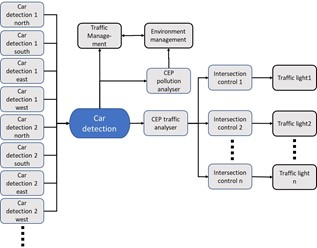
\includegraphics[width=0.7\linewidth]{Figures/Chapter5/figuresshared/SharedInputPoolEvent.jpg}
	\caption[Shared Input Pools and Complex Event Processing]{Shared Input Pools and Complex Event Processing}
	\label{fig:sharedInputPoolEvents}
\end{figure}






\section{Hierarchies in Communication Oriented Business Process Models}
PASS  offers powerful possibilities for structuring complex process systems. The ways to do that are demonstrated with an example.
As an example we will consider a process for realizing a car break down service. This service con-sists of several connected processes. There is the main process for handling the car accident and supporting e.g. processes for organising towing and repair shop services. Insurance companies may be involved for covering damages, the customer gets an invoice, uses money transfer services or banks for paying the invoice. These processes are executed by various organisations like help desk service companies, towing service companies, car repair workshops banks etc.. In most business process projects not complete processes are described in detail only a certain part is considered e.g. only the help desk process has to be considered in detail but to do that we have to considere the whole environment in which a considered process is embedded. We have to know which rela-tions exists to these other processes. It is necessary to know which inputs are rquired by neighbour processes and which results they deliver. A help desk process which organizes the towing services has to know how the towing service is requested and which further interactions are required. For instance it must be agreed whether the towing service informs the client about the arrival time of the towing truck or the help desk does it.


\subsection{Process Architecture}

Rectangles represent processes. Each process has a name. Processes consists of other processes and/or subjects. The lines between the rectangles represent the communication channels between processes. Each communication channel has a nameand can contain other communication chan-nels and/or messages.

Figure \ref{fig:car-service-level1} shows the highest process level of the car break down service. In the "car use" process the event "car break down" happens. In order to organize support an interaction is initiated with process "car break down service" . Between these processes messages are exchanged which are elements of the communication channel "Car break down handling".\\


\begin{figure}[ph]
	\centering
	
\includegraphics[width=0.7\linewidth]{Figures/Chapter5/figures-hierarchy/Car-Service-Level1.jpg}
	\caption[High level structure of car break down service]{High level structure of car break down service}
	\label{fig:car-service-level1}
\end{figure}



Figure \ref{fig:car-service-leve2} shows the next process structure level of the process "car break down ser-vice". In this level the process "Car break down service" is separated in 10 processes. The processes "Bank", "Insurance service", "Car repair workshop", "Incident Management","Mobility Manage-ment" and "Towing Management" have a communication channel to the prcess "Car usage". This means the communication channel "Car break down handling" is separated into five communica-tion channels. Each of them covers the communication with the relared process, e.g. the communi-cation channel "Accident notification Car break down" is the communication channel between the processes "Car usage" and "Incident Management".\\


\begin{figure*}
	\centering
	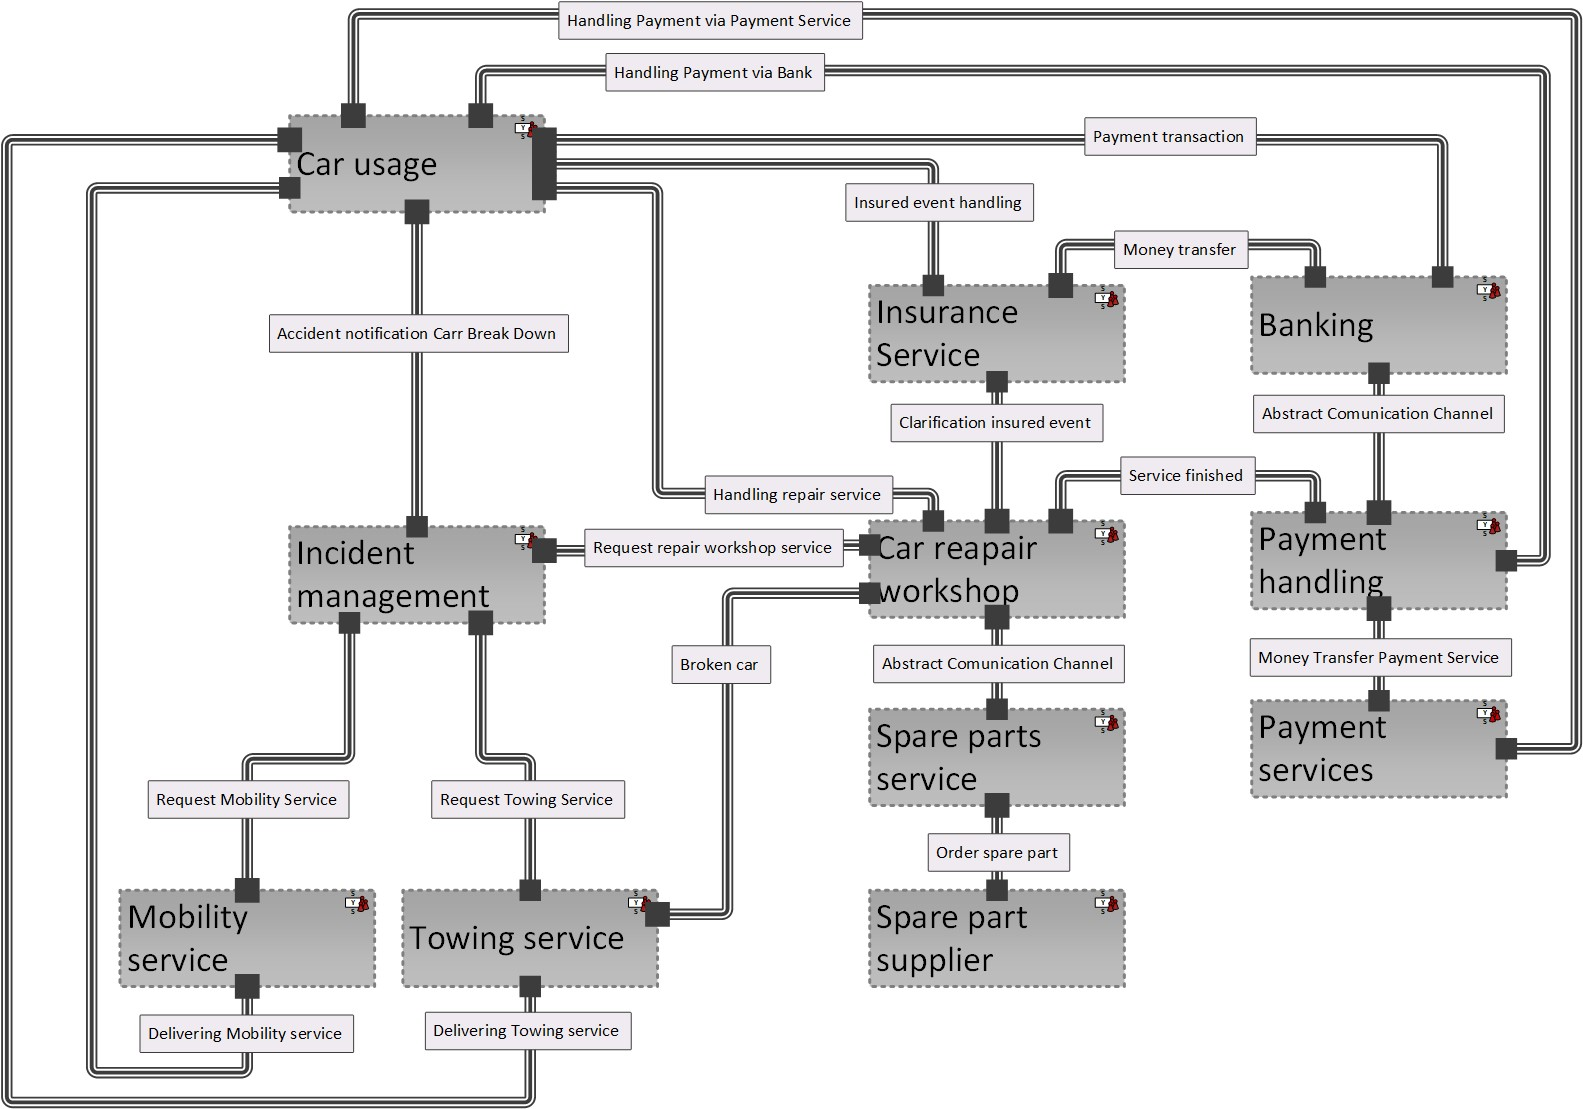
\includegraphics[width=0.8\linewidth]{Figures/Chapter5/figures-hierarchy/Car-Service-Leve2}
	\caption[Structure of the Emmergency Call Handling Process]{Structure of the Emmergency Call Handling Process}
	\label{fig:car-service-leve2}
\end{figure*}



Inside a process there can be also processes. This means that levels of processes can be built. Figure \ref{fig:car-service-lev3} shows the next deeper level of our process hierarchy. The process "Car repair workshop" is structured in six processes. According to this separation the communication sets are also splitted e.g. the communication set "Handling repair service" is splitted into three parts, one part is han-dled by the process "Service scheduling" the other by the process "Car droping" and the third one by the process "Customer Satisfaction".\\

\begin{figure*}
	\centering
	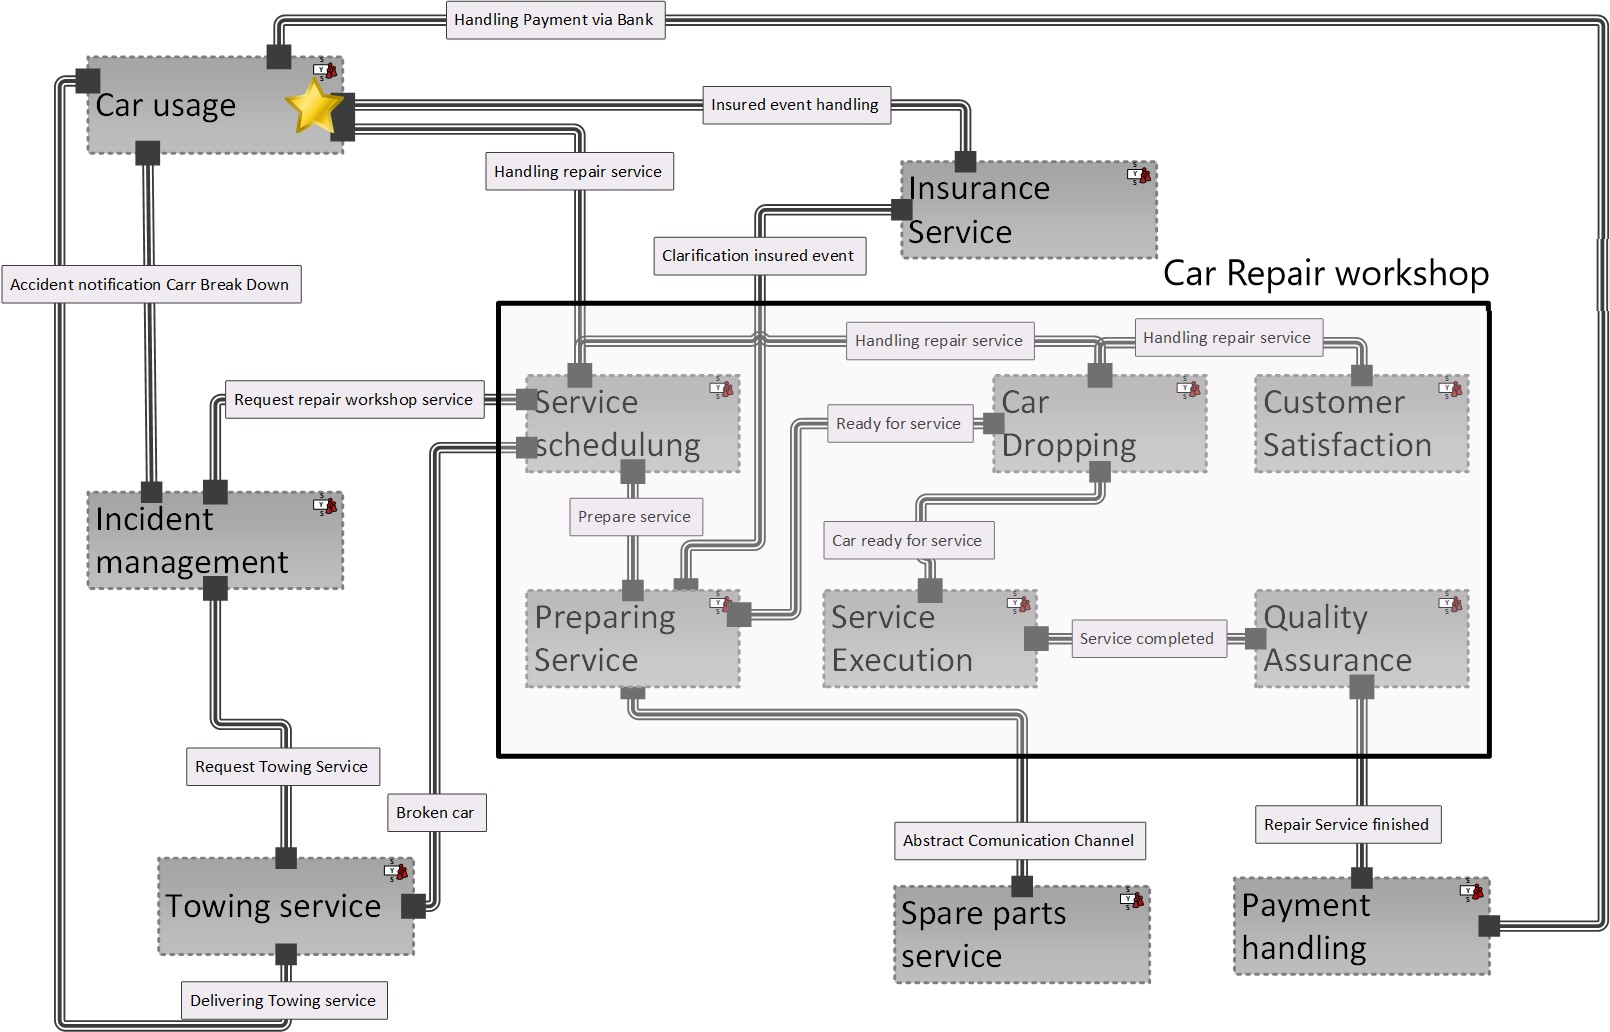
\includegraphics[width=0.8\linewidth]{Figures/Chapter5/figures-hierarchy/Car-Service-Lev3}
	\caption[Details of the "Car repair workshop" Process]{Details of the "Car repair workshop" Process}
	\label{fig:car-service-lev3}
\end{figure*}

As already mentioned, processes cannot communicate directly with each other. The active entities of a process, the subjects communicate with each other. This means messages from one process are sent to an other process are reveived by a subject inside of that process. Messages belonging to a channel are assigned to a sending or receiving subject at the lowest level of an process architecture. This lowest level of a process description is the subject interaction diagram (SID) which shows the involved subjects of a process and the messages they exchange. In the following we consider the process incident management in more detail. This process does not contain other processes like the process "Car Repair Shop". The process "Incident management" contains a Subject Interaction Diagram. Some of the subjects of a process communicate with subjects in other processes. These subjects are called border subjects because they are at the border of a process to other prcesses. Figure \ref{fig:car-service-lev4} shows the process "Incident management" with its border subjects. There is a border subject "Help agent" which communicates with the processes "Towing service", "Mobility ser-vice"and  "Car repair workshop", precisely it communicates with a subject in one of these process-es. Another border subject of the process "Incident management" which is called "Help desk"communicates with the process "Car usage".\\

\begin{figure}[ph]
	\centering
	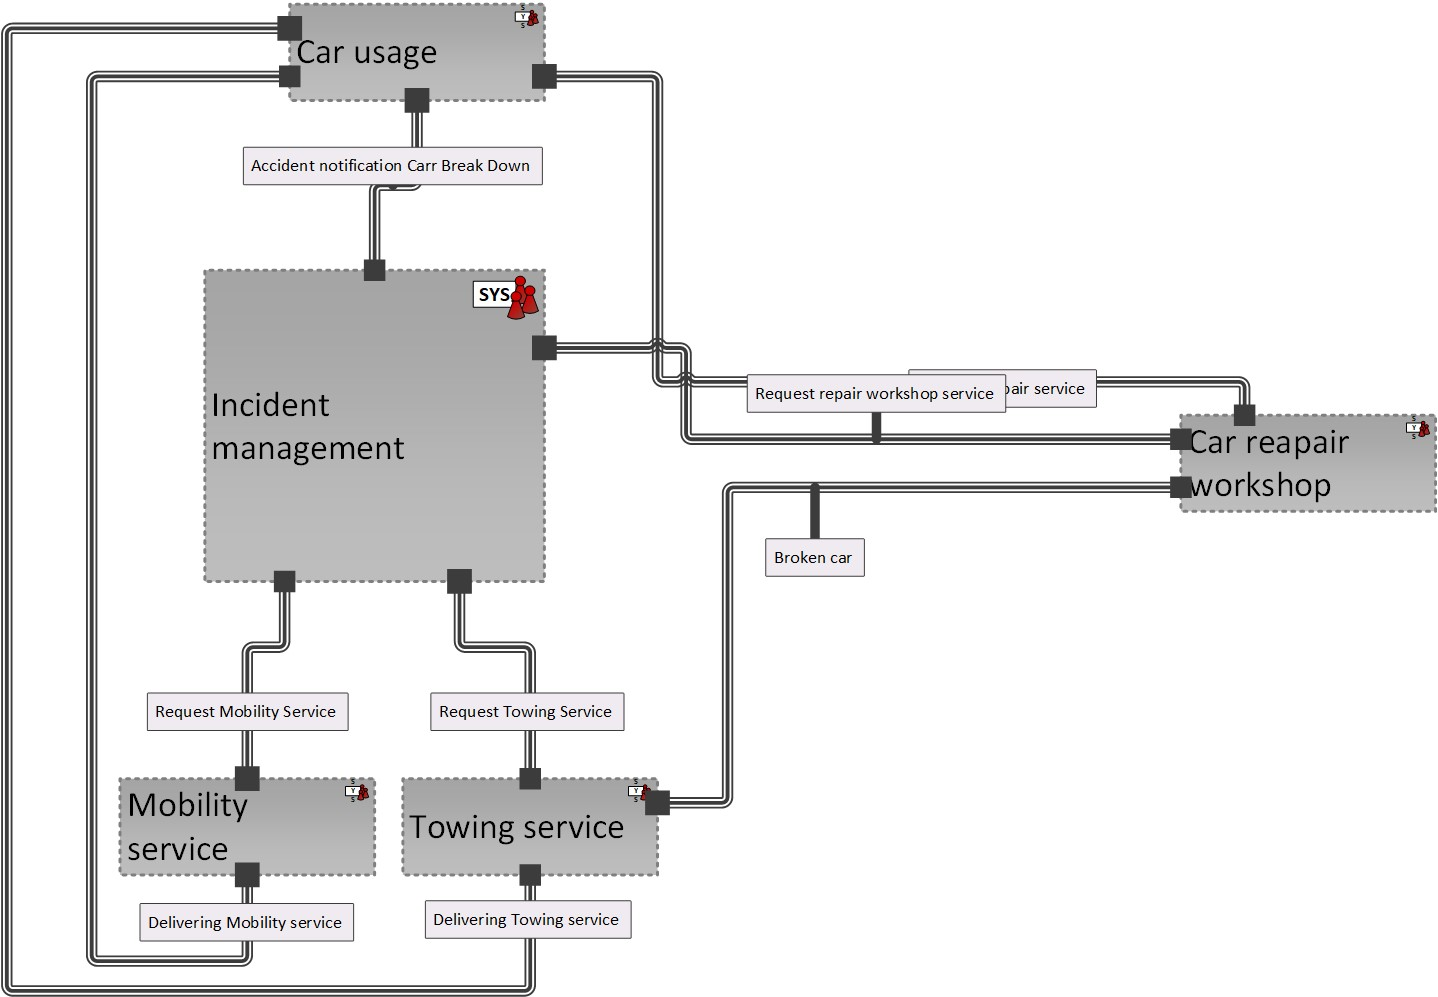
\includegraphics[width=0.9\linewidth]{Figures/Chapter5/figures-hierarchy/Car-Service-Lev4}
	\caption[Neighbors of the "Incident Manaement Process"]{Neighbors of the "Incident Manaement Process"}
	\label{fig:car-service-lev4}
\end{figure}

The border subjects of the process "Incident management" must have a coresponding border sub-ject at the neighbour processes. The border subjects "Call agent" communicates with the border subject "Help requestor" of process "Car usage" and the border subject "Help agent" communi-cates with border subjects of the processes "Car repair workshop", "Towing service and "Mobility service". The process "Incident management" with all the border subjects is shown in  figure \ref{fig:car-service-lev5}.\\

\begin{figure}
	\centering
	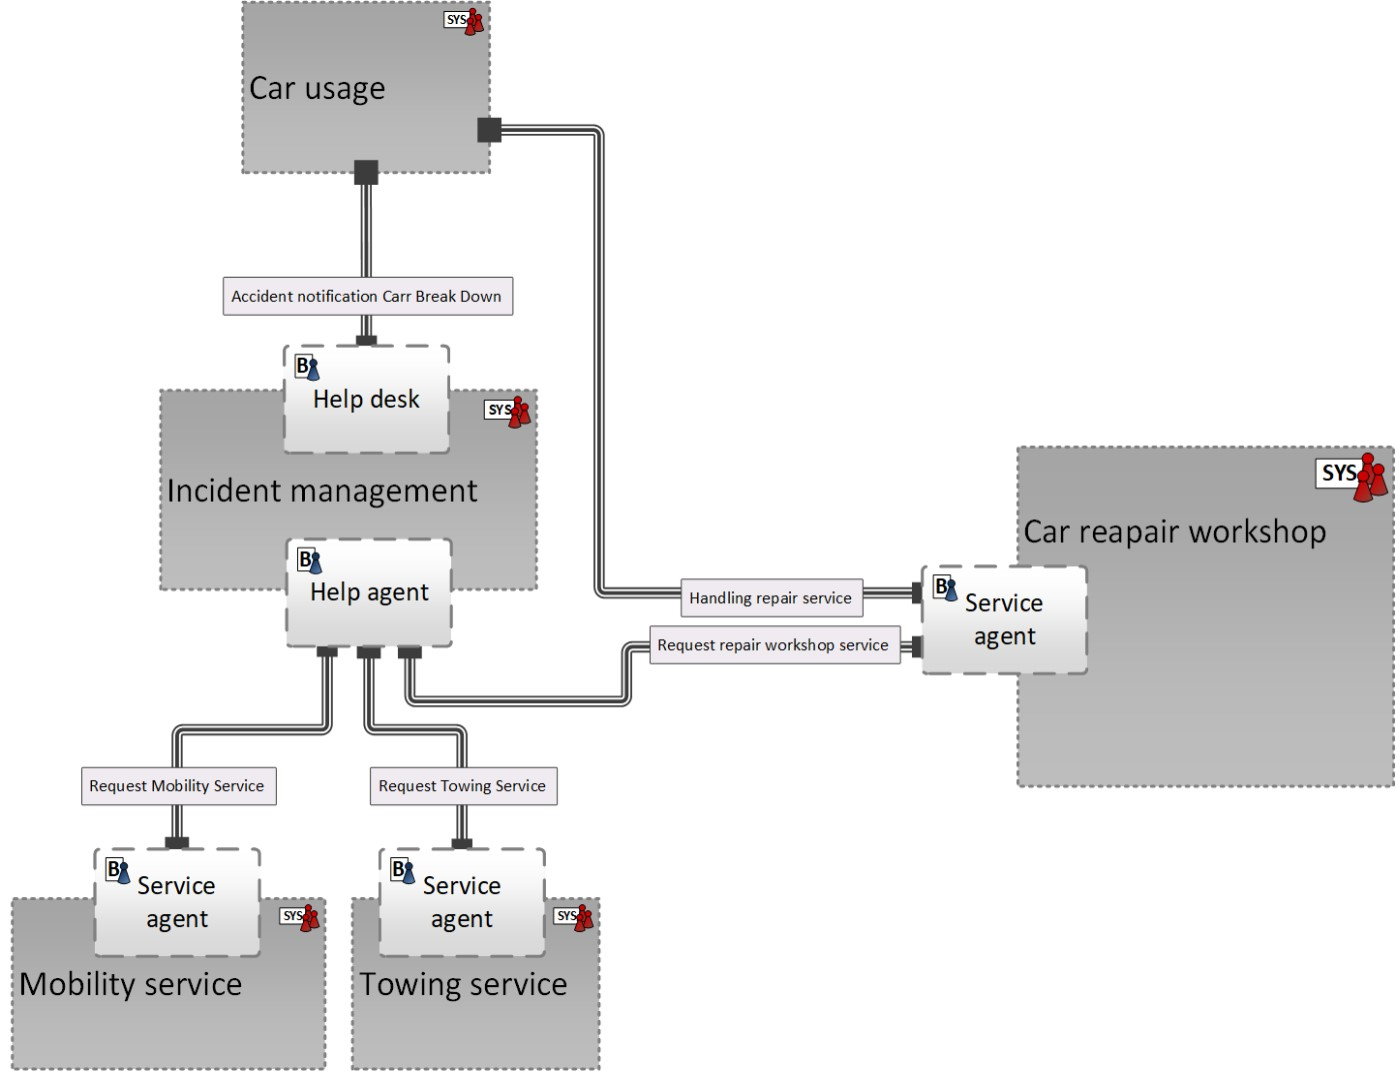
\includegraphics[width=0.9\linewidth]{Figures/Chapter5/figures-hierarchy/Car-Service-Lev5}
	\caption[Border subjects of the "Incident Management" Process]{Border subjects of the "Incident Management" Process}
	\label{fig:car-service-lev5}
\end{figure}

The border subjects of the processes "Mobility service", "Towing service" and "Car repair work-shop" have the same name “Service agent” but these are different subjets because they belong to different processes. Because the process "Car repair workshop" consists of several layers the corre-sponding border subject can be in a process which is part of process "Car repair workshop" in a lower level.\\
From the perspective of the subjects inside of the process "Incident managent" are the border subjects of the processes "Mobility service", "Towing service" and "Car repair workshop" interfaces to these processes, therefore they are called interface subjects in the subject interaction diegram of a process. Figure \ref{fig:car-service-lev6}shows the subject interaction diagram of the process incident management.\\


\subsection{Behavioral Interface}
Processes to which a considered process has communication relationships are called process neighbours or for short neighbours. Now we want to consider the details of the communication relationships between two neighbours. The interface between two processes is defined by the related border subjects and the allowed sequences in which the messages a communication channel are exchanged between them. As already described above each message is defined by a name and the data which are transported the so-called payload. A border subject observes the behavior of the border subject of the neighbour process and vice versa. Figure \ref{fig:car-service-lev8} shows the border subject "Help desk" of the processes "Incident Management" which communicates with the border subject of process "Car usage".\\

\begin{figure}
	\centering
	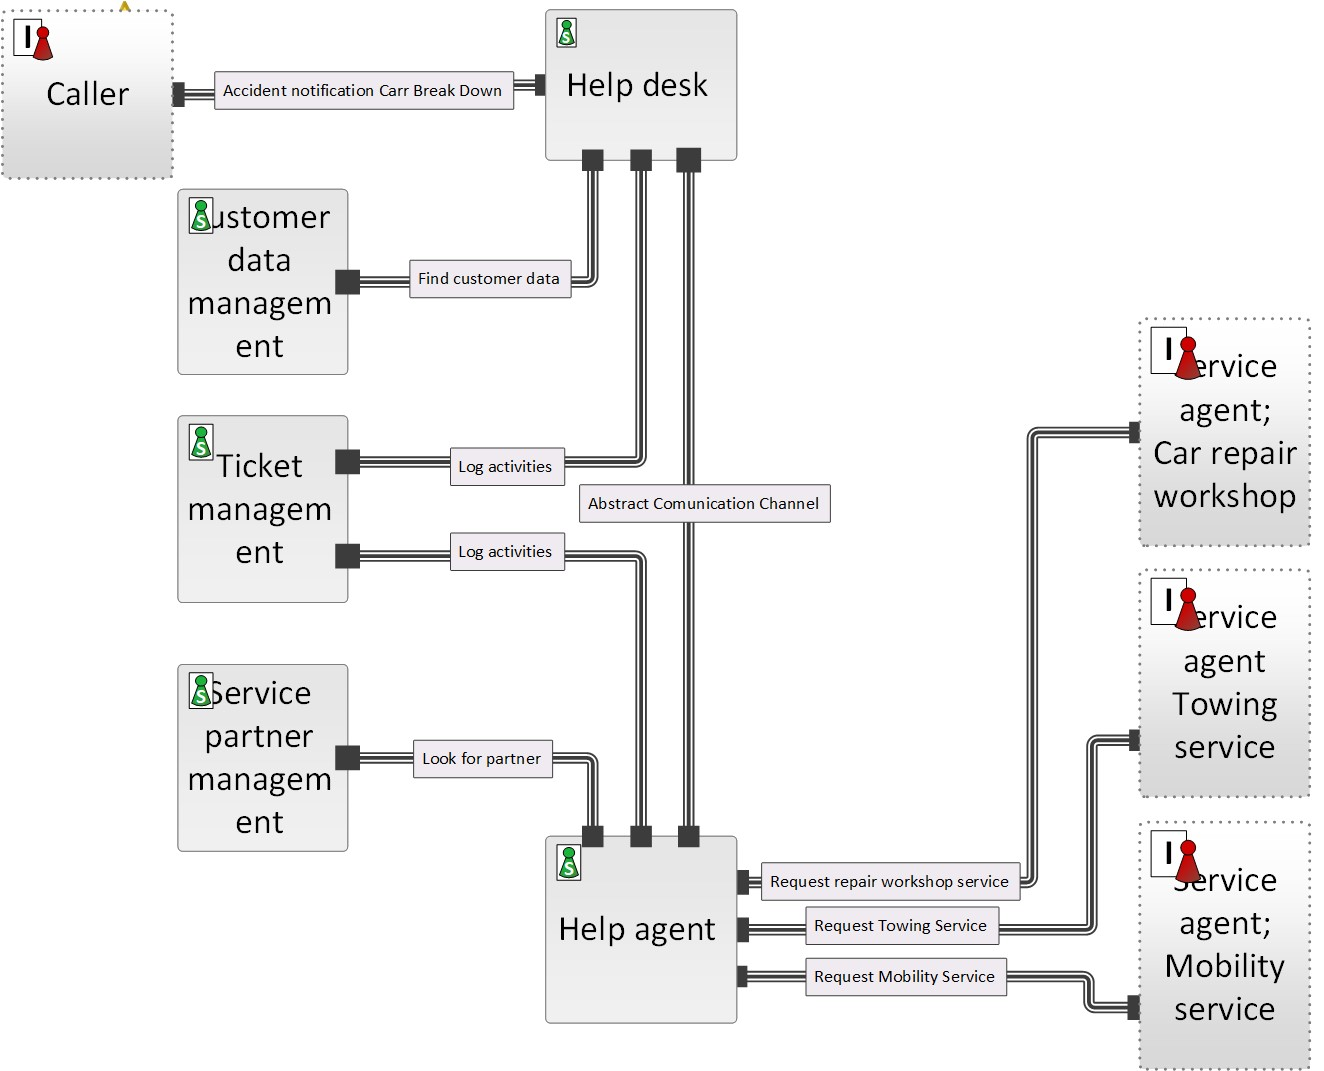
\includegraphics[width=1.0\linewidth]{Figures/Chapter5/figures-hierarchy/Car-Service-Lev6}
	\caption[Subject Interaction Diagram of the Process "Incident Management"]{Subject Interaction Diagram of the Process "Incident Management"}
	\label{fig:car-service-lev6}
\end{figure}

Because we consider the process "Incident management" the border subject "Caller" of the process "Car usage" becomes an interface subject in the SID (details about interface subjects can be found in \cite{Flei12}) of the process “Incident Management”. Figure \ref{fig:car-service-lev8} shows the detailed subject interaction diagram around the subject help desk. \\

\begin{figure}
	\centering
	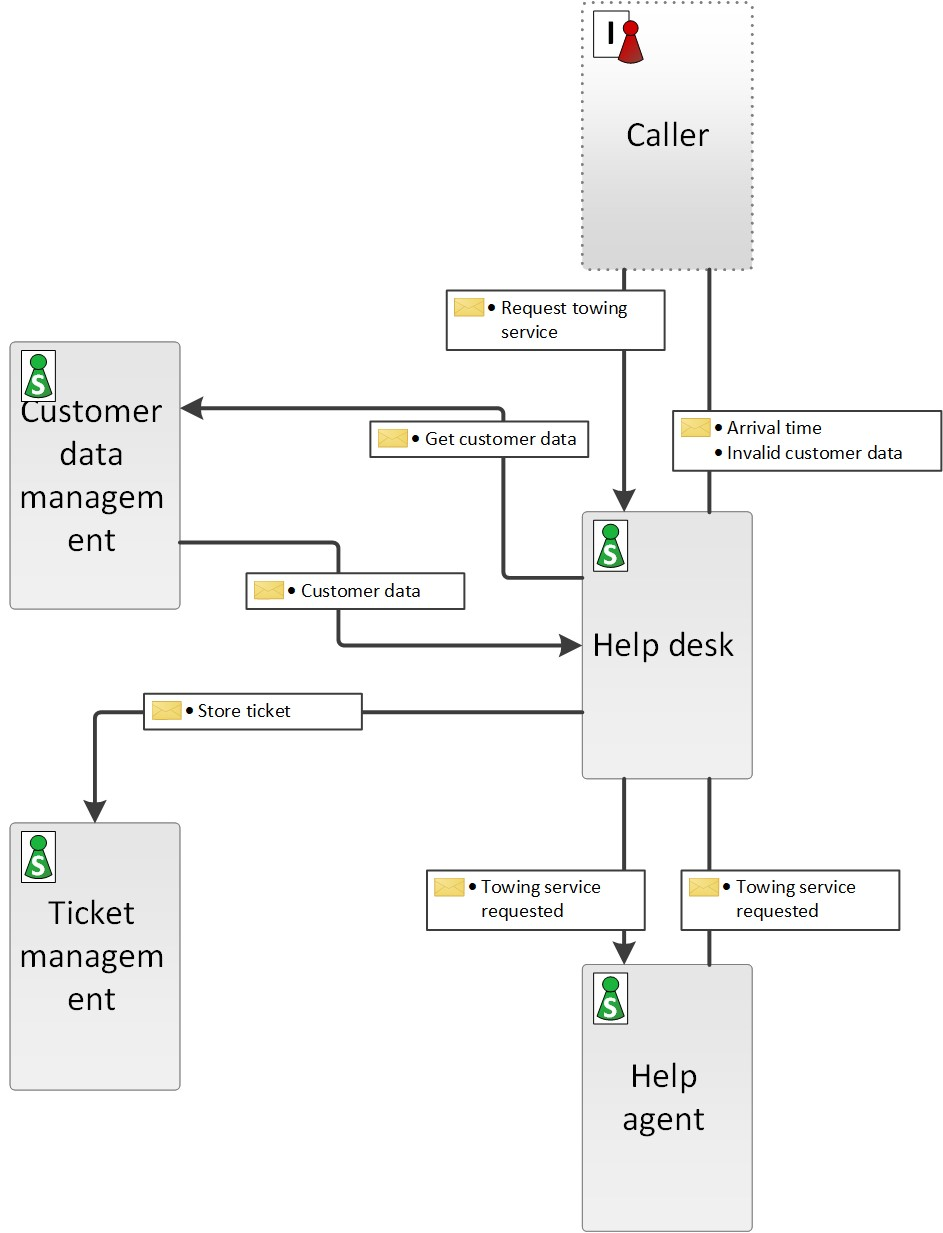
\includegraphics[width=0.9\linewidth]{Figures/Chapter5/figures-hierarchy/Car-Service-Lev8}
	\caption[Subject Interaction around the subject “Help desk”]{Subject Interaction around the subject “Help desk”}
	\label{fig:car-service-lev8}
\end{figure}

Instead of the channels the messages required for a towing service request are shown. A message "Request towing service" comes from the interface subject. This message is accepted by the subject "help desk". The subject help desk checks the customer data received with this message by sending a corresponding the message "Get customer data" to the subject "Customer data management". This subject send the complete customer data back to the subject "Help desk" via the message "Customer data". The subject "Help desk" checks the customer data. If the data are invalid a message "Invalid customer data" is sent to the subject "Caller" and the process is finished.\ 
If the customer data are valid with that data the subject "Help desk" creates a trouble ticket which is sent to the subject "Ticket management". After that the message "Towing service requested" is sent to the help agent which organizes the towing service. The part of the communication structure of the subject "Help agent" in order to organize the towing service is not shown in figure \ref{fig:car-service-lev9}. We only see that subject "Help agent" sends the message "Towing service data" to the subject "Help desk". This message contains all the data about the service e.g. name of the towing company and arrival time. The subject "Help desk" forwards that data to the interface subject "Caller". This behavior is shown in figure \ref{fig:car-service-lev8}.\\



\begin{figure}
	\centering
	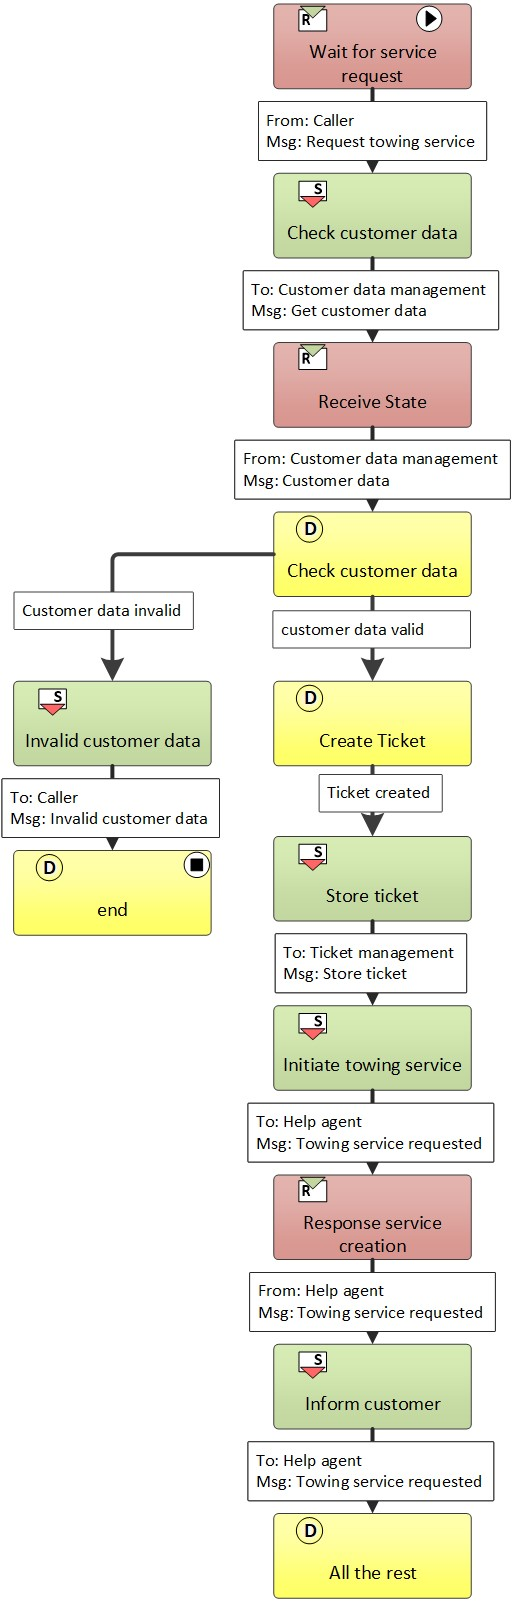
\includegraphics[width=0.7\linewidth]{Figures/Chapter5/figures-hierarchy/Car-Service-Lev9}
	\caption[Part of the Behavior Diagramm of the subject “Help desk”]{Part of the Behavior Diagramm of the subject “Help desk”}
	\label{fig:car-service-lev9}
\end{figure}


The behavior described in the figure above contains the communication with all neighbor subjects of subject "Help desk" including the communication with the interface sub-ject "Caller". From the perspective of this subject the communication of the subject "Help desk" with its other neighbor subjects is not relevant. For the subject "Caller" only the commumication sequence between itself and the subject "Help desk" is relevant. These allowed communication sequences are called the behavioral interface.\\
The behavioral interface between two subjects can be derived from the complete behavior of a subject by deleting the interactions with all the other subjects . Figure \ref{fig:car-service-lev10} shows how the communication sequence relevant for the communication be-tween the subject "Help Desk" and "Caller" is derived from the complete behavior of subject "Help desk".

\begin{figure}
	\centering
	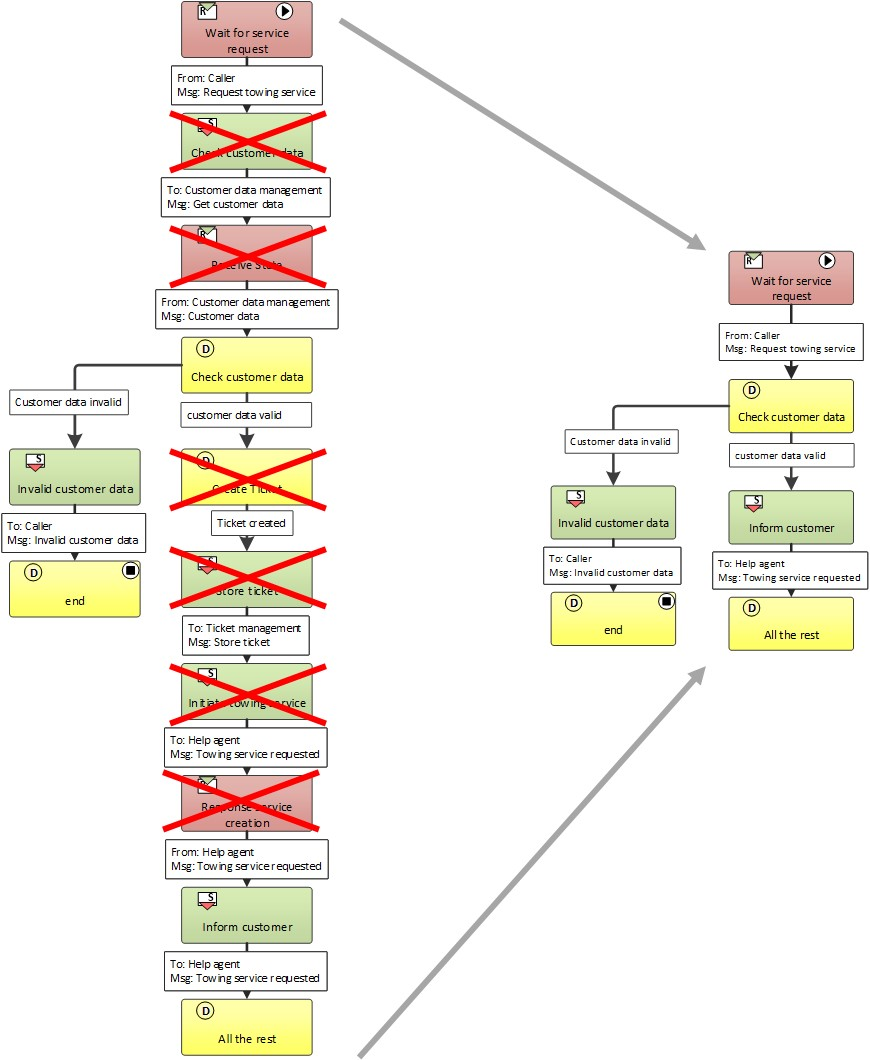
\includegraphics[width=1.0\linewidth]{Figures/Chapter5/figures-hierarchy/Car-Service-Lev10}
	\caption[Deriving the Behavioral Interface from the Subject Behavior]{Deriving the Behavioral Interface from the Subject Behavior}
	\label{fig:car-service-lev10}
\end{figure}

A behavoral interface is always relative to a communication partner. In figure \ref{fig:car-service-lev10} the behavioral interface is relative to the interface subject "Caller". The behavioral interface to the subject "Ticket Management" is different because only the communication activities with this subject are considered.This behavioral interface would be very simple. It consists of only one send activity, sending the message "Store ticket".\\
The behavioral interface relative to a partner subject can be automatically derived from the complete behavior of a subject
(see \cite{article:jCPEX}).


\section{Business Activity Monitoring for S-BPM}

Monitoring of Business Process looks at running instances. For those it measures metrics, aggregates them to Process Performance Indicators (PPIs) as a business process-related form of Key Performance Indicators (KPIs), reveals deviations (as-is vs. to-be) and report and presents results to people in charge or interested in the value of the PPI. Thus monitoring lays ground for the performance analysis in the key dimensions quality, time and costs of processes and helps identifying weaknesses and opportunities for improvement \cite{book:UntPerform}.
By feeding back information for completed and running instances to analysis monitoring fosters organizational learning, forms an important part of the Business Process Management (BPM) lifecycle \cite{article:SUbjetorientiertBPM} and thus helps implementing the operational level in the closed-loop approach to enterprise performance management \cite{book:processmonitoring} (see \ref{fig:Approach-Performance}).

\begin{figure}[h]
	\centering
	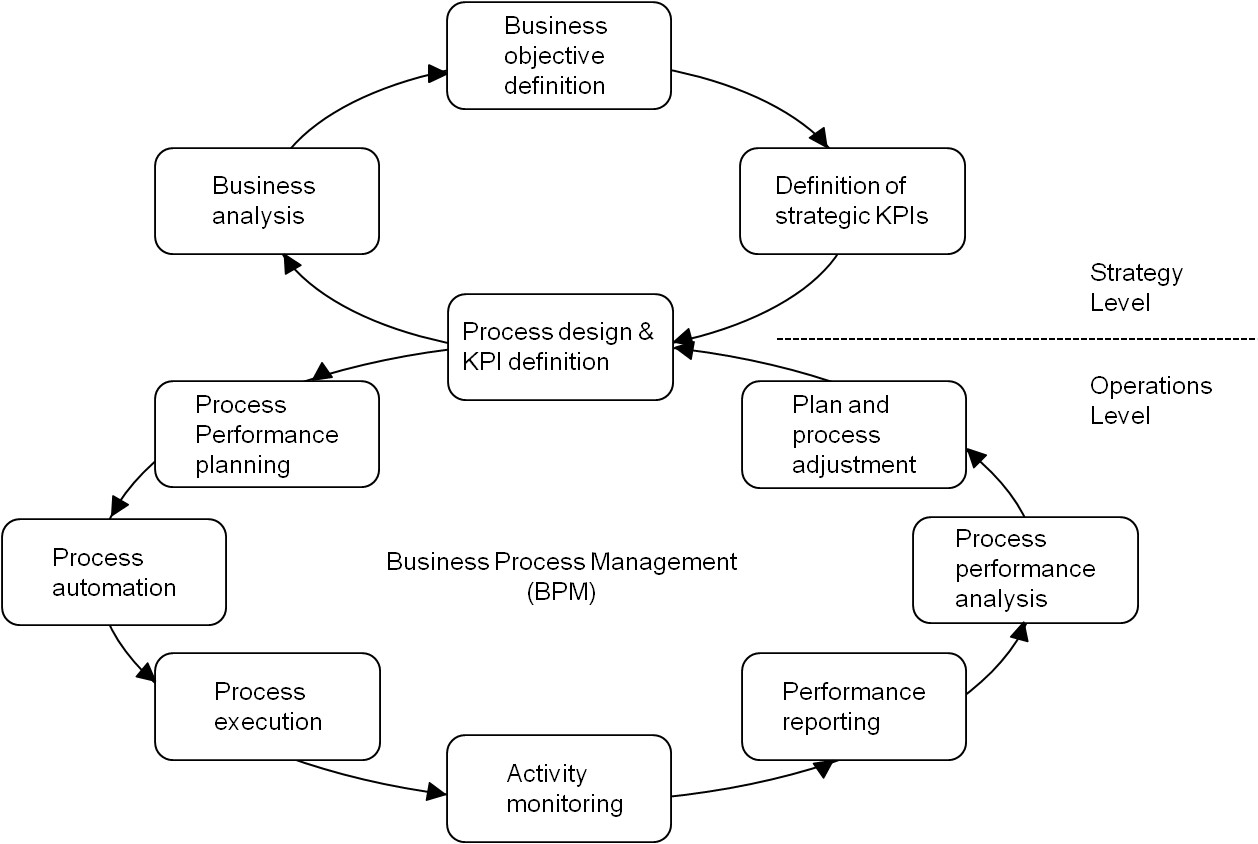
\includegraphics[width=0.9\linewidth]{Figures/Chapter5/Monitoring/Approach-Performance-Mgmt.jpg}
	\caption[Closed-loop Approach to Performance Management]{Closed-loop Approach to Performance Management [6]}
	\label{fig:Approach-Performance}
\end{figure}



\subsection{Architecture }  
A Business Activity Monitoring (BAM) environment supported by Complex Event Processing consists of several elements necessary at build time and at runtime (see \ref{fig:BAMArchitecture}) [27, 8, 15]. At build time a modeling environment should provide tools for designing processes (e.g. Metasonic Build) and defining process performance indicators (PPIs), BAM events, rules, thresholds etc. as well as parameters for their visualization in report and on dashboards. At runtime there are (1) event producers like a process engine (e.g. Metasonic Flow) or an ERP system (e.g. SAP) which feed events into an event cloud or stream (chronologically ordered). (2) Event Processing Agents (EPA) form the event processing logic. They process events based on metrics, event patterns, rules and other parameters specified at design time. Their basic logical functions include filtering and transforming events and detecting patterns among them. Global state elements allow them accessing data from outside the application (e.g. from an ERP system). EPAs put the results of their processing (also to be understood as events) out to Event Consumers (3) like dashboards or process engines. Input and Output Adapters (IA, OA) transform event data between different formats of system elements as necessary. All system elements involved form an Event Processing Network (EPN), in which events are exchanged by communication mechanisms.

\begin{figure}[h]
	\centering
	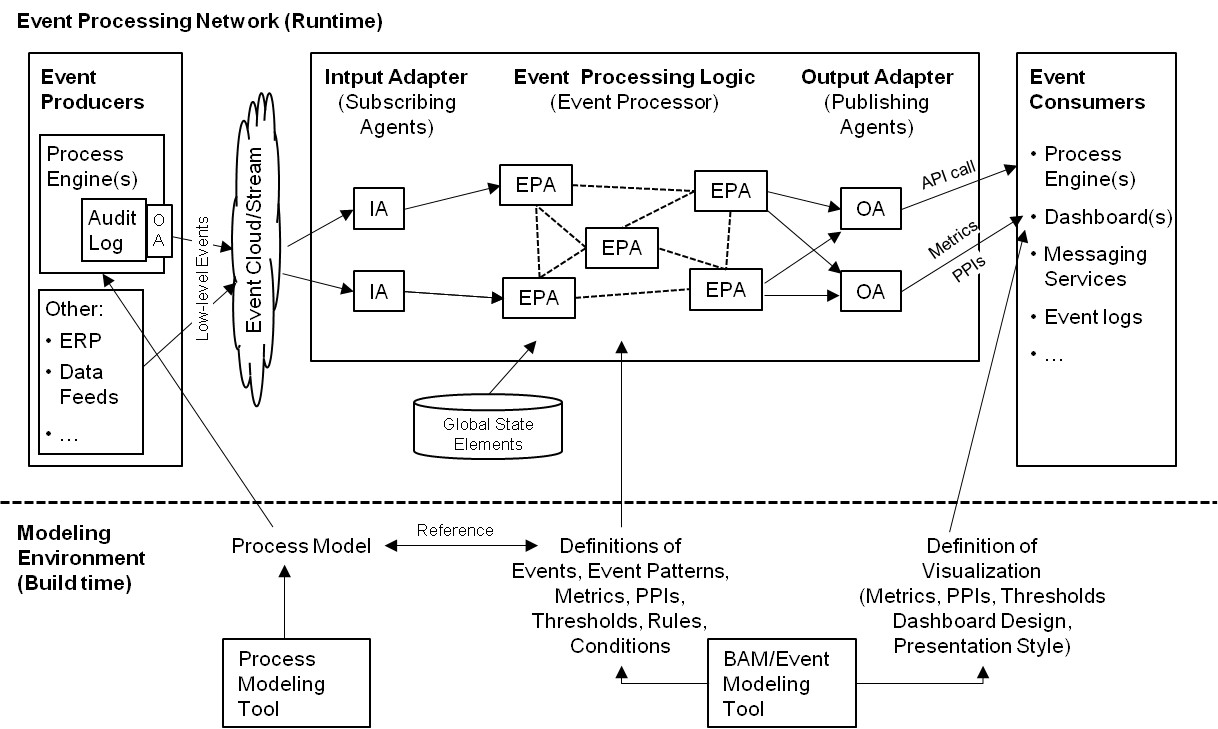
\includegraphics[width=0.9\linewidth]{Figures/Chapter5/Monitoring/Integrated-BAM-CEP-Architecture-27.jpg}
	\caption[Integrated BAM/CEP Architecture 27]{Integrated BAM/CEP Architecture [27]}
	\label{fig:BAMArchitecture}
\end{figure}



\subsection{Modeling BAM Parameters at Build Time}
As mentioned in the last section it is necessary not only to model the processes, but also numerous pieces of information relevant for a sound process monitoring in the sense of Business Activity Monitoring (BAM model). These can be derived from answers to questions like what, when, how and how often should be measured by whom [25]. The information should also include how single metrics are to be aggregated in order to determine Process Performance Indicators (PPIs). For systematically collecting and documenting the necessary information fact sheets or templates for metrics and performance indicators have been developed [17, 20]. \ref{tbl:Fact-Sheet}  shows an extract of a sample fact sheet defined for the average processing time of activities (see also [31, 23]).


\begin{table}[htbp]
	\footnotesize
	\centering
	\begin{tabular}[t]{@{}l p{0.5\linewidth} p{0.3\linewidth} @{}}
		\toprule
		\textbf{Attribute} & \textbf{Content}  \\
		\midrule
		 & \textbf{Characteristics}
		\\
		Identifier & Average activity time
		\\
		Description & Average time of a process activity within a certain period
		\\
		To-be value/unit & tbd specifically (min.)
		\\
		Tolerance range/unit & tbd specifically (\%)
		\\
		Escalation Rules/ Actions & In case of violation alert the process owner and start escalation process (tbd specifically)
		\\
		Addressees & Process Owner, Middle Mangement, Accountants (tbd specifically)
		Responsibility	Process Owner (tbd specifically)
		\\
		&  &
		\\
		& \textbf{Measuring and Computing}
		\\
		Measuring Object & All instances of the process 'Purchase Order'
		\\
		(Single) Metrics & Start time and end time of all activities of the process
		\\
		Measuring Method & Read time stamps for beginning and end of activities written by Metasonic Flow 
		\\
		Measuring Frequency & For every single instance as it occurs
		\\
		Algorithms & For computing period: Sum of processing time of all activities divided by number of instances

		\\
		Data Sources (general) & Tables in the database of Metasonic Suite:
		RT\_PROCDESC, RT\_PROCINST, REC\_PARADESC, REC\_RECTRANS, UM\_USER
		\\
		Data Sources (specific) & Activity processing time (for one instance):\newline
		\textbf{SELECT} TIMESTAMP1  \newline
		(\textbf{SELECT} STARTTIME \newline
		\textbf{FROM} RT\_PROCINST \newline
		\textbf{WHERE} RT\_PROCDESC = \textit{process (purchase order)}\newline
		\textbf{AND} ID = \textit{instance (9)}\newline
		\textbf{FROM} REC\_RECTRANS\newline
		\textbf{WHERE} RT\_STDESC = \textit{\textit{state (fill\_in\_form)}}\newline
		\textbf{AND} RT\_PROCINST = \textit{instance (9)}
		Completed instances: see separate fact sheet .
		\\
		Computing Period (time, no. of inst.) & Daily
		\\
		& &
		\\
		& \textbf{Presentation}
		\\
		Presentation Style & As-is value and to-be value in combination with a spark line showing the historical development, deviation from to-be value in \%
		\\
		Presentation Frequency & Weekly and in case of escalation
		\\
		Archiving & Stored in additional database table, linked with RT\_PROCDESC
		\\
		
\bottomrule
\end{tabular}
\caption{Fact Sheet for a PPI (extract)}
\label{tbl:Fact-Sheet}
\end{table}

Replacing the content column by more formal ontology-based linguistic patterns as suggested by Del-Río-Ortega et al. (see table 2) could help relating PPIs to elements of the process model, performing automated analysis [5] and implementing the measurement at runtime. 

\begin{table}[htbp]
	\footnotesize
	\centering
	\begin{tabular}[t]{@{}l p{0.3\linewidth} p{0.4\linewidth} p{0.5\linewidth} @{}}
		\toprule
		\textbf{Attribute} & \textbf{Linguistic Pattern}  & \textbf{Example}\\
		\midrule
		PPI-<ID> & <PPI descriptive name> & PPI-001 Average time of RFC analysis
		\\
		Process	& <process ID the PPI is related to> & Request for change (RFC)
		\\
		Goals & <strategic or operational goals the PPI is related to> & BG-002: Improve customer satisfaction \newline
		BG-014: Reduce RFC time to response
		\\
		Definition & The PPI is defined as { \newline
			<DurationMeasure> | <CountMeasure> | <ConditionMeasure> |
			<DataMeasure> | <DerivedMeasure> | <AggregatedMeasure> }
		[expressed in <unit of measure>] & The PPI is defined as the average of Duration of Analyse RFC activity
		\\
		Target & The PPI value must { \newline
			be {greater | lower} than [or equal to] <bound> | \newline
			be between <lower bound> and <upper bound> [inclusive] |\newline
			fulfil the following constraint: <target constraint> } & The PPI value must be slower than or equal to 1 working day
		\\
		Scope & The process instances considered for this PPI are {
			the last <n> ones |
			those in the analysis period <AP-x> } & The process instances considered for this PPI are the last 100 ones
		\\
		Source & <source from which the PPI measure can be obtained> &	Event logs of BPMS
		\\
		Responsible & { <role> | <department> | <organization> | <person> } &	Planning and quality manager
		\\
		Informed &{ <role> | <department> | <organization> | <person> } & CIO
		\\
		Comments & <additional comments about the PPI> & Most RFCs are created after 12:00
		\\
\bottomrule
\end{tabular}
\caption{PPI Template based on Linguistic Patterns [5]}
\label{tbl:Fact-Sheet-PPI}
\end{table}


Friedenstab et al. argue that such linguistic patterns do not fit to the usually graphical modeling of processes which makes integration difficult [12]. The authors discuss some more approaches to BAM modeling. With regard to the limitations revealed, they present a BAM-related extension of the graphical Business Process Model & Notation (BPMN) [12].
Using an abstract language syntax based on the Unified Modeling Language (UML) they started defining meta models for language constructs needed for BAM as there are Duration, Frequency, Composed Basic Measure, Aggregated Measure, Filter, Target Definition, Actions, Measure-based Expressions and Dashboard. Figure 8 depicts the example for the duration of elements on different levels of detail, where the grey colored parts indicate references to the BPMN specification.

\begin{figure}[h]
	\centering
	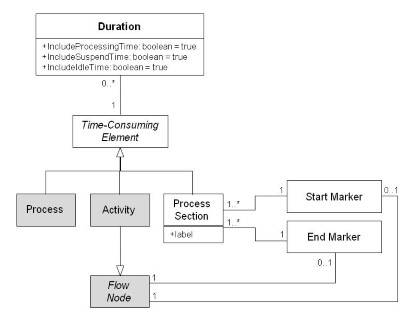
\includegraphics[width=0.9\linewidth]{Figures/Chapter5/Monitoring/Meta-Mode-fo-Duration-relate-to-BPMN-1.jpg}
	\caption[Meta Model for Duration (related to BPMN) 12]{Meta Model for Duration (related to BPMN) [12]}
	\label{fig:Meta-Model}
\end{figure}


In a second step Friedenstab et al. developed a concrete syntax allowing for modeling the abstract language elements with graphical symbols and text labels. Parts of it are visible in figure 9. The example shows the BAM model for determining the cycle times of a purchase order process modeled in BPMN (lower part). The upmost part for example expresses the fact that the overall cycle time (Duration) for the last 50 instances (Filter) has to be determined and displayed on the dashboard (Dashboard). Monitoring the average of the overall cycle time for completed instances controls the modeled business logic of the process. If it is above 48 hours goods are delivered with an express shipping if the average cycle time is more than. Otherwise standard shipping is carried out. A deviation also leads to an alert sent to the process owner, while in any case the average is to be presented on the dashboard. The latter is also valid for the third time-related metric in the example, the partial cycle-time for the company-internal part of the process, which is set into relation with the overall cycle time.

\begin{figure}[h]
	\centering
	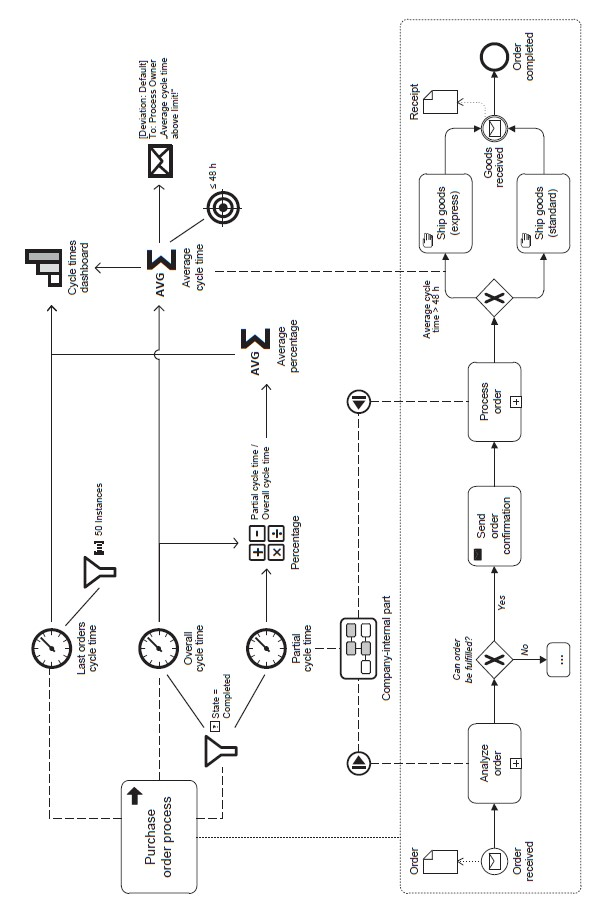
\includegraphics[width=0.9\linewidth]{Figures/Chapter5/Monitoring/BAM Model for Cycle Times.jpg}
	\caption[BAM Model for Cycle Times of a Purchase Order Process based on BPMN 12]{BAM Model for Cycle Times of a Purchase Order Process based on BPMN [12]}
	\label{fig:Model-Cycle-Times}
\end{figure}


The concept presented by Friedenstab et al. is thoroughly thought-out and clearly and precisely elaborated. The idea now is to adapt it to Subject-oriented Business Process Management and relate the abstract syntax to the S-BPM meta model instead of BPMN. Due to S-BPM being a more precise and comprehensive notation than BPMN [2] the mapping should be possible without problems. Table 3 compares the BPMN specification elements used by [12] with the ones appropriate in S-BPM [9].
Table 3.  BPMN and S-BPM Specifications used in BAM Constructs
BAM Language Syntax Construct	Used BPMN Specification Element 	Suitable S-BPM Specification Element 
Duration
(Time-Consuming Element)	Process, Activity, Flow Nodes	Process, Subject Behaviour States (Function, Send, Receive, Start, End)
Frequency
(Countable Element)	Process, Activity, Data Objects, Data States	Process, Subject Behaviour States (Function, Send, Receive), Business Objects and their States
Actions	Process	Process
Measure-based Expressions	Expression, Sequence Flow	Incoming Message

The remaining constructs as well as the extensions do not depend on the process modeling language and thus are not included in the table.
On the other hand S-BPM, following its paradigm of regarding subjects, predicates and objects as equally important parts of a process, offers the subject as an additional specification element to add . In figure 10 we modified the picture of figure 8 by replacing the BPMN by S-BPM elements and adding the subject. This allows modeling the determination of the overall time a subject (respectively the allocated resource(s)) spends on working on a process instance. This is of interest for cost-related analysis (see section 2.3).

\begin{figure}[h]
	\centering
	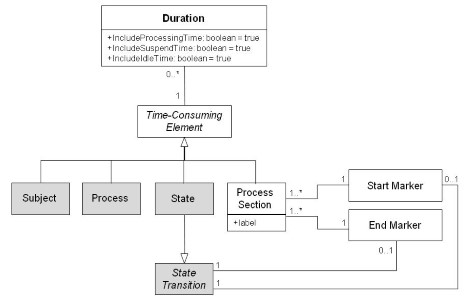
\includegraphics[width=0.9\linewidth]{Figures/Chapter5/Monitoring/Meta-Mode-fo-Duration-relate- to-SBPM.jpg}
	\caption[Meta Model for Duration (related to S-BPM)]{Meta Model for Duration (related to S-BPM)}
	\label{fig:Meta-Model-S_BPM}
\end{figure}



Fig. 10. Meta Model for Duration (related to S-BPM)

In order to show how the BAM language syntax constructs can be related to subject-oriented models we designed the purchase order process in S-BPM. Due to missing information in the BPM model some assumptions were necessary like who performs the process steps (subjects). We then added the BAM modeling symbols to create a monitoring model similar to that in figure 9.
The result is depicted in the following graph. In the lower part it includes the subject interaction diagram (SID) of the process. The SID shows the subjects involved and how they coordinate themselves in the course of action by exchanging messages. In the monitoring model in the upper part a difference can be seen. The partial cycle time for the company-internal activities can be modeled by just relating the clock symbol to the subject ‘Sales’. In the example this subject represents all steps carried out within the organization. In the same way we can determine the cycle time for the other subjects.

\begin{figure}[h]
	\centering
	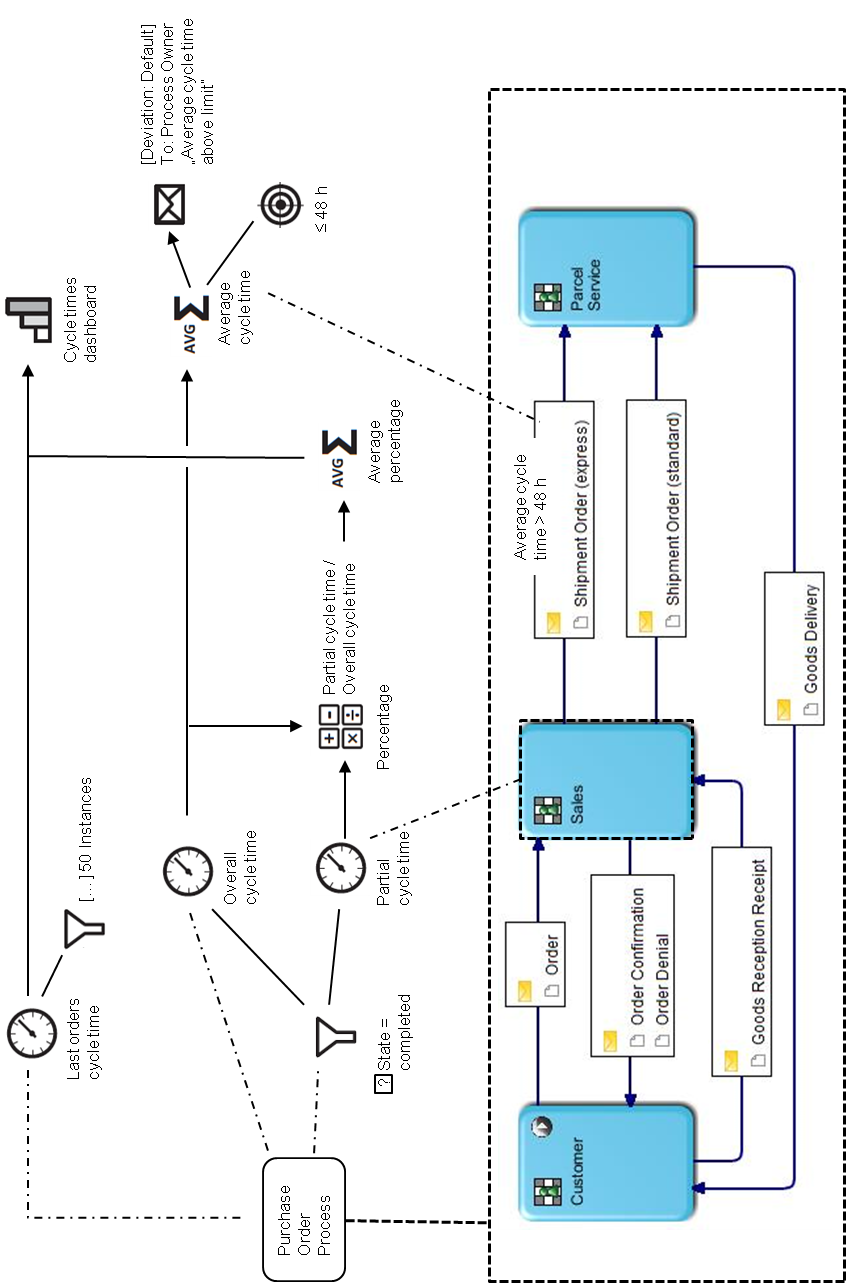
\includegraphics[width=0.9\linewidth]{Figures/Chapter5/Monitoring/BAM-Model-fo- Cycle-Times-of-a-Purchase-Order-Process-based-on-S-BPM.png}
	\caption[BAM Model for Cycle Times of a Purchase Order Process based on S-BPM]{BAM Model for Cycle Times of a Purchase Order Process based on S-BPM}
	\label{fig:Cycle-Time-SBPM}
\end{figure}


Fig. 11. BAM Model for Cycle Times of a Purchase Order Process based on S-BPM
Given a special information demand a more granular modeling of BAM parameters is possible on the subject behavior level. Figure 12 for example details the behavior of ‘Sales’ including all receive, send and functional states walked through by the subject. The symbols indicate that the average cycle time between order reception and confirming the order to the customer should be measured. In the same way cycle times between states in behaviours of different subjects can be modelled.


\begin{figure}[h]
	\centering
	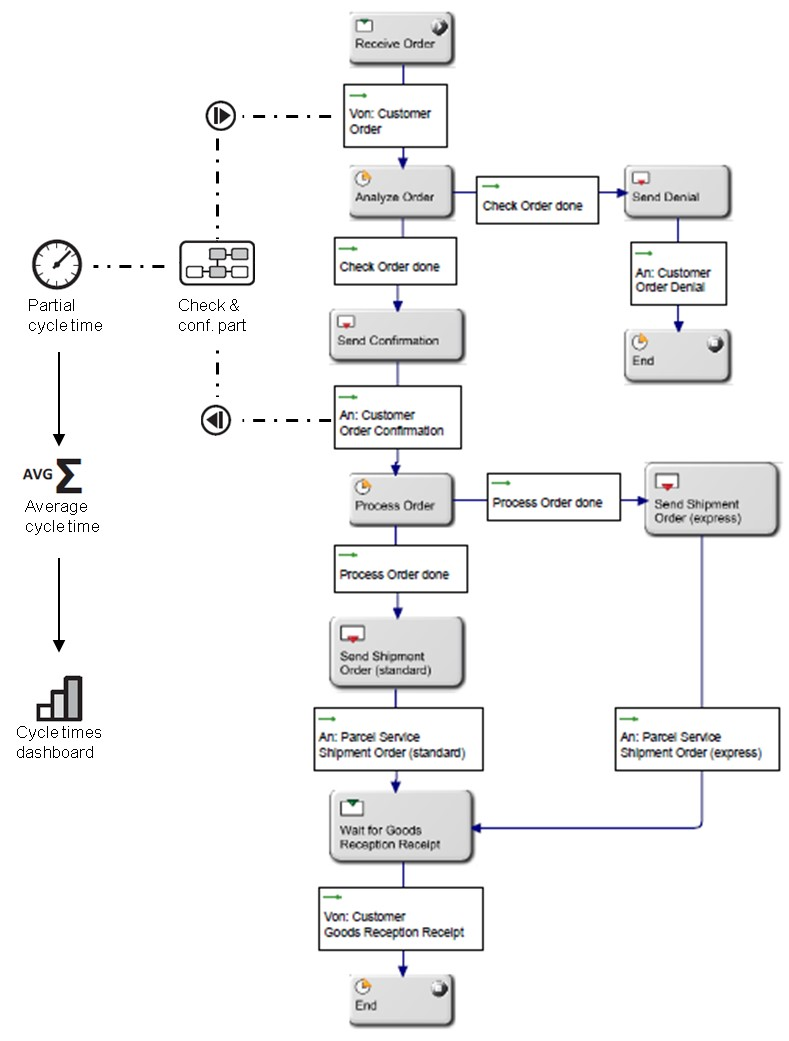
\includegraphics[width=0.9\linewidth]{Figures/Chapter5/Monitoring/BAM-Model-for-Cycle-Time-of-a-Process-Section-based-on-S-BPM.jpg}
	\caption[BAM Model for Cycle Time of a Process Section based on S-BPM]{BAM Model for Cycle Time of a Process Section based on S-BPM}
	\label{fig:BAM-Cycle-Time}
\end{figure}

\ref{fig:BAM-Cycle-Time}Fig. 12. BAM Model for Cycle Time of a Process Section based on S-BPM
Back on the level of subject interaction diagram we could also model to determine the overall time for receiving (waiting), sending and doing, both by process and by subject. Modeling on the two diagram levels reduces complexity.
4   Conclusion and future Work
This contribution systematized Business Process Monitoring and shed some light on the current state of monitoring in the context of S-BPM. Starting there we emphasized Business Activity Monitoring and took a closer look to the modelling of BAM parameters. We showed that the approach for BPMN presented by Friedenstab et al. can be adapted to S-BPM with little effort and that S-BPM shows additional potential to further develop the concept.
This is where future work needs to continue. The first step to go should be elaborating, detailing and tailoring the modeling language for the needs of S-BPM in order define a comprehensive basis for the succeeding task of developing easy-to-use software tool support. These could be pursued as parts of the Open S-BPM Initiative, which is underway to develop – among other artifacts - a process modeling and a process execution software for S-BPM, both based on the Eclipse Ecore meta model (see [11, 14] and http://www.i2pm.net/open-s-bpm/projects). The BAM modeling tool should make use of the model data created by the process modeling tool and add its results to a combined model base both for process execution and BAM. The third step would then be to build BAM functionality which at runtime processes events according to the subject-oriented BAM models. There is some evidence that S-BPM provides good premises to support event processing [10], e.g. by integration of a CEP Engine or single Event Processing Agents as subjects into processes. This has to be proven by a thorough investigation of the interrelationship and integration potential of CEP and S-BPM concepts and solutions. Generating code for BAM functionality out of the BAM model is another challenge to tackle [12]. With the clear formal semantic of its underlying process algebra the S-BPM modeling language allows this for process models [9]. Consequently it seems to be worthwhile to investigate the possibilities of code generation out of BAM models too. 
\\
\\
\\
\textbf{References}\\
\\
\textbf{\textit{The references have to be inserted in a general bibliography and the coresponding refernces have to be replaced in this section.}}\\
\\
1.	Accorsi, R., Ulrich, M., Van der Aalst, W.: Process Mining, Informatik Spektrum, Band 35, Heft 5, 2012, pp. 354-359.
\\
2.	Börger, E.: Approaches to modeling business processes: a critical analysis of BPMN, workflow patterns and YAWL, Journal of Software and Systems Modeling, Vol. 11 (3) 2012, pp. 305-318.
\\
3.	Chandy, K., Schulte, W.: Event Processing: Designing IT Systems for Agile Companies, New York, 2010.
\\
4.	DeFee, J., Harmon, P.: Business Activity Monitoring and Simulation, in: Fischer, L. (ed.), Workflow Handbook, Future Strategies Inc., Lighthouse Point, 2005, pp.53-74.
\\
5.	Del-Río-Ortega, A., De Reyna, M., Durán Toro, A., Ruiz-Cortés, A.: Defining Process Performance Indicators by Using Templates and Patterns, in: Barros, A., Gal, A., Kindler, E. (eds.): BPM 2012, LNCS 7481, Springer, Berlin Heidelberg, 2012, pp. 223-228.
\\
6.	Dinter, B., Bucher, T.: Business Performance Management, in: Chamoni, P., Gluchowski, P. (Eds.), Analytische Informationssysteme, 3rd Ed., Springer, Berlin Heidelberg, 2006, pp. 23-50.
\\
7.	Eckert, M., Bry, F.: Complex Event Processing (CEP), Informatik Spektrum, Band 32, Heft 2, 2009, pp. 163-167.
\\
8.	Etzion O., Niblett P.: Event Processing in Action, Manning Publications, Stamford, 2011.
\\
9.	Fleischmann, A., Schmidt, W., Stary, C., Obermeier, S., Börger, E.: Subject-oriented Business Process Management, Springer, Berlin Heidelberg, 2012.
\\
10.	Fleischmann, A., Schmidt, W., Stary, C., Strecker, F.: Nondeterministic Events in Business Processes, Proceedings of the 6th International Workshop on Event-driven Business Process Management (edBPM2012), co-located with BPM 2012, Tallinn/Estonia, Lecture Notes in Business Information Processing (LNBIP), Springer, Berlin Heidelberg, 2012
\\
11.	Fleischmann, A., Schmidt, W., Stary: Open S-BPM, in: Fischer, H., Schneeberger, J. (Eds.), Proceedings of the 5th International Conference S-BPM ONE 2013, Communications in Computer and Information Sciences (CCIS) No. xxx, Springer, Berlin Heidelberg 2013.
\\
12.	Friedenstab, J.-P., Janiesch, C., Matzner, M., Müller, O.: Extending BPMN for Business Activity Monitoring, 45th Hawaii International Conference on System Sciences, 2012, pp. 4158-4167.
\\
13.	Heß, H.: Von der Unternehmensstrategie zur Prozess-Performance – Was kommt nach Business Intelligence? in: Scheer, A.-W., Jost, W., Heß, H. und Kronz, A., Corporate Performance Management, Berlin, 2005, pp. 7-29.
\\
14.	Institute of Innovative Process Management (I2PM), www.i2pm.net.
\\
15.	Janiesch, C., Matzner, M., Müller, O.: A Blueprint for Event-driven Business Activity Management, in: Rinderle, S., Toumani, F., and Wolf, K. (Eds.), 9th International Conference on Business Process Management (BPM). LNCS 6896, Springer, Berlin Heidelberg, 2011, pp. 17-28.
\\
16.	Kang, J., Kwan, H.: A Business Monitoring System Supporting Real-Time Business Performance Management, Proceedings of the 2008 Third International Conference on Convergence and Hybrid Information Technology (ICCIT '08) Vol. 1, Washington DC 2008, pp. 473-478.
\\
17.	Kütz, M.: Kennzahlen in der IT: Werkzeuge für Controlling und Management. 3. Aufl., dpunkt, Heidelberg, 2009.
\\
18.	Luckham, D., Schulte, R. (Eds.): Event Processing Glossary Version 2.0/2011, Event Processing Technical Society, http://www.complexevents.com/2011/08/23/ event-processing-glossary-version-2-0/, last access 2012-07-25.
\\
19.	Luckham, D.: The Power of Events: An Introduction to Complex Event Processing in Distributed Enterprise Systems, Amsterdam, 2002.
\\
20.	Marx Gómez, J., Junker, H., Odebrecht, S.: IT-Controlling, Erich Schmidt Verlag, Berlin 2009.
\\
21.	Metasonic Flow, User Manual V4.4, Metasonic AG, www.metasonic.com, Pfaffenhofen, 2012.
\\
22.	Panagos, E., Rabinovich, M.: Predictive Workflow Management, Proceedings of the 3rd International Workshop on Next Generation Information Technologies and Systems, 1997, pp. 193-197.
\\
23.	Pehlke, A.: Aufbau eines Business Activity Monitoring für den subjektorientierten Ansatz des Business Process Managements (S-BPM), Bachelor Thesis, University of Applied Sciences Ingolstadt, Ingolstadt 2012.
\\
24.	Petzel, E., Czaja, R., Simulation-based Process Optimization, in: Fischer, H., Schneeberger, J. (Eds.), Proceedings of the 5th International Conference S-BPM ONE 2013, Communications in Computer and Information Sciences (CCIS) No. xxx, Springer, Berlin Heidelberg 2013.
\\
25.	Schmelzer, H., Sesselmann, W.: Geschäftsprozessmanagement in der Praxis, 7. Auflage, Hanser, München, 2010.
\\
26.	Schmidt, W., Fleischmann, A. und Gilbert, O.: Subjektorientiertes Geschäftsprozess-management, HMD – Praxis der Wirtschaftsinformatik, Heft 266, 2009, pp. 52-62.
\\
27.	Schmidt, W.: Business Activity Monitoring, in: Rausch, P., Sheeta, A., Ayesh, A., Business Intelligence and Performance Management - Theory, Systems and Industrial Applications, Springer UK, 2013.
\\
28.	Schulte, W., Gassman, B.: Business Activity Monitoring, in: Dixon, J. (ed.): Hype Cycle for Business Process Management 2012. Gartner Inc. 2012, pp. 92-94.
\\
29.	Van der Aalst, W.: Process Mining, Springer, Berlin Heidelberg, 2011.
\\
30.	Von Ammon, R. Ertlmaier, T., Etzion, O., Kofman, A., Paulus, T.: Integrating Complex Events for Collaborating and Dynamically Changing Business Processes in: Dan, A., Gittler, F. and Toumani, F. (Eds.): ICSOC/ServiceWave 2009, LNCS 6275, Springer, Berlin Heidelberg, 2010, pp. 370–384.
\\
31.	Zehbold, C., Schmidt, W., Fleischmann, A.: Activity-Based Costing for S-BPM, in: Fischer, H., Schneeberger, J. (Eds.), Proceedings of the 5th International Conference S-BPM ONE 2013, Communications in Computer and Information Sciences (CCIS) No. xxx, Springer, Berlin Heidelberg 2013.
\\
32.	Zehbold, C.: Controllingansatz für S-BPM, Working Papers Series of the University of Applied Sciences Ingolstadt, No. 25, Ingolstadt, 2012.


\section{Subject Oriented Project Management}

\section{Subject Oriented Project Management}

